\subsection{Chapter Overview}

\subsection{Experimentation Setup}

An energy baseline model will be developed for the following machines, at $10$ and $30$ minute time aggregations, to analyze EE and perform PDD: main terminal, main ventilation, paper disposal, uv server room, and uv ground floor. The implementation of Gaussian Process Regression is with the open source package GPyTorch \cite{gardner2018gpytorch}; a highly efficient and modular implementation of GPs built on top of PyTorch, with graphical process unit (GPU) acceleration. 

As multiple machines, each with two time aggregations, are being modeled, an experimentation workflow is introduced to track and log results pertaining to the evaluation metrics outlined in \hyperlink{subsection.3.7}{Section 3.7} and the GP kernel design described in \hyperlink{subsection.3.6}{Section 3.6}. The flowchart in \hyperlink{figure.11}{Figure 11} provides the overview for the experimentation setup. 

Starting at the top, a machine's measurement data provided by CLEMAP's meters is queried where an EDA is performed similar to that in \hyperlink{subsubsection.4.2.1}{Section 4.2.1}. Subsequently, the GP model and kernel design begins using the results from the EDA as our prior belief. Here, kernels pertaining to cyclical patterns and local variations are designed. At the same time, the data set is split into a training and validation set. The training set, representing data from $11.10.2021$ - $15.10.2021$, is used for the optimization of the kernel hyperparameters. For optimization, the gradient-based method ADAM (adaptive moment estimation) \cite{pml1Book} is used at different learning rates (lr) and iterations (see \hyperlink{table.3}{Table 3} for results). Then, with the optimized hyperparameters, inference is performed using the posterior predictive distribution. The composite kernel is decomposed into its individual kernel components to analyze the effect of each kernel. This decomposition allows one to investigate if increasing the model complexity (by introducing more  kernels) contributes to a decrease or increase in uncertainty (using Pinball loss). Lastly, the evaluation metrics are calculated on the predictions $\hat{y}$ and test data $y_{test}$ and logged in the database. Based on these metrics, it is determined if further kernel designs and or model refinements need to be tested. If yes, then repeat, else save model parameters and end process. The end of this workflow results in an energy baseline model ready for analyzing EE and performing PDD for the given machine.   

\begin{figure}[H]
\centering
\graphicspath{ {./images/} }
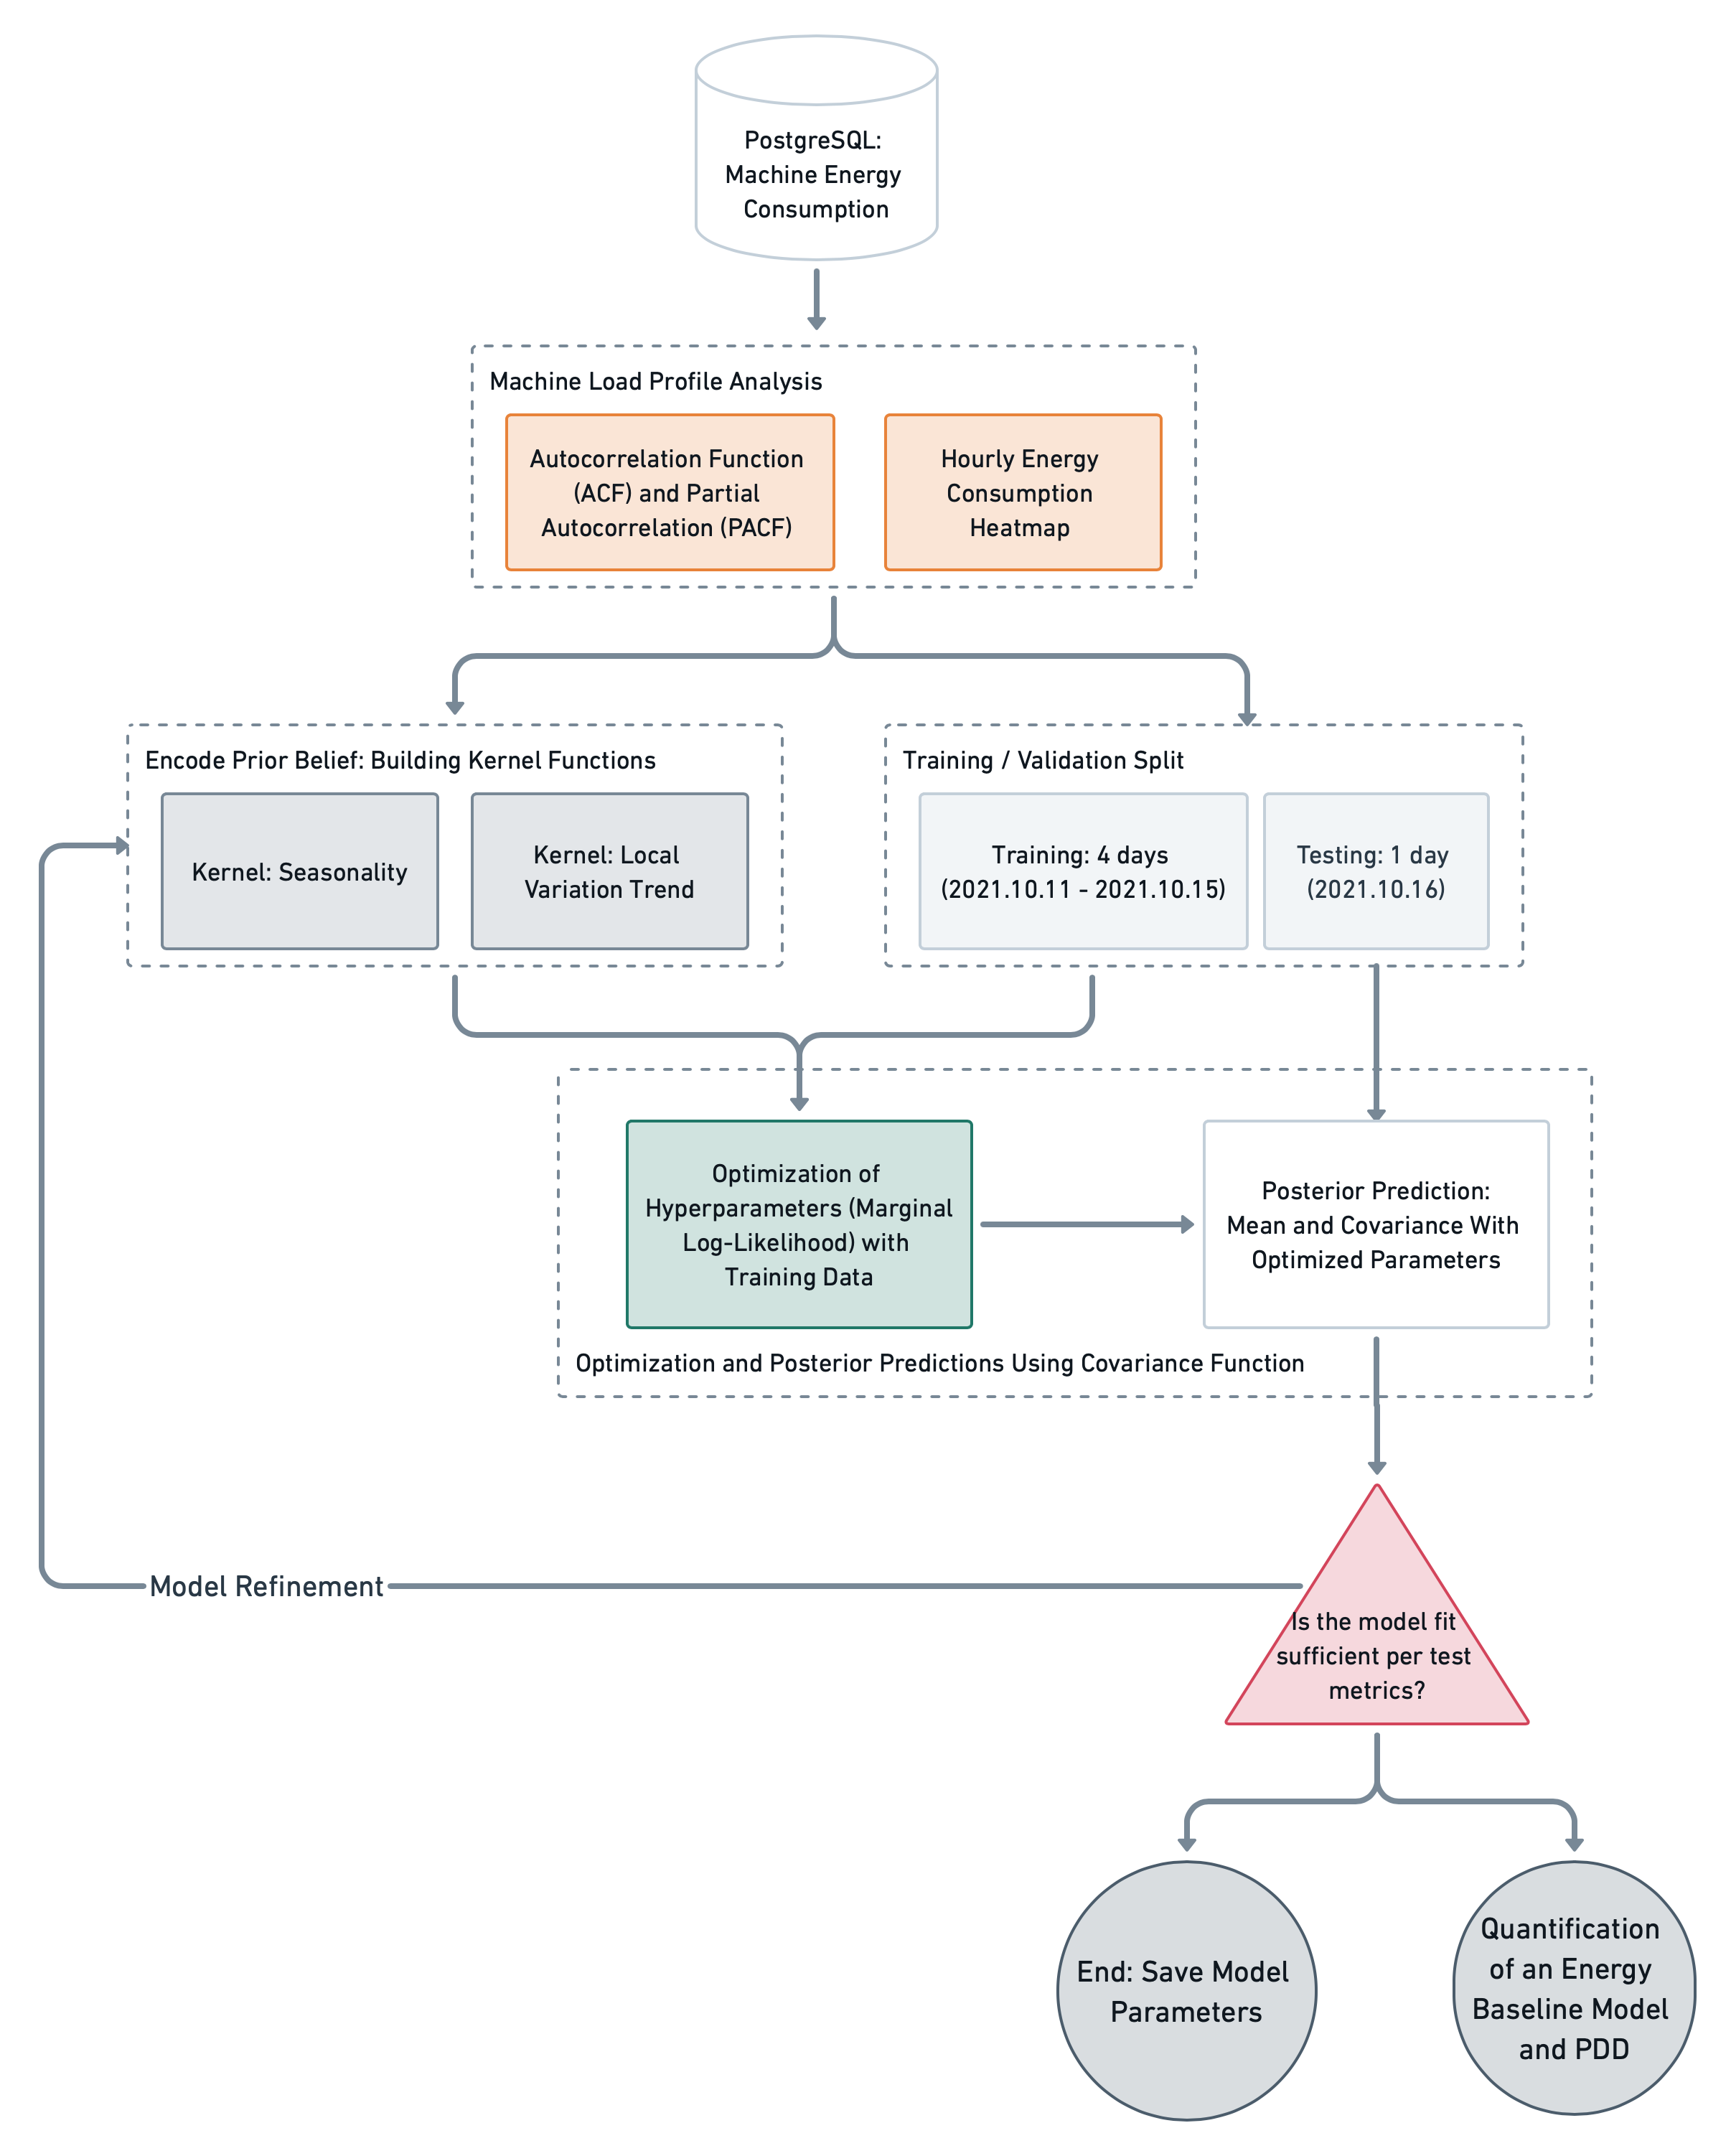
\includegraphics[scale=0.32]{images/experiment_flow.png}
\caption{Experimentation workflow for developing and refining GP energy baseline models.}
\end{figure}

\subsection{Kernel Design and Composition}

In this section, the kernel design is outlined for the paper disposal machine using the results from the EDA and kernels described in \hyperlink{subsection.3.5}{Section 3.5}. Recall that the GP model uses time as input and kW (Watts / $1000$) as the output. Before the kernel design and composition is outlined, a particularity of GP models is the normalization and or standardization of data before hyperparameter optimization. Thus, the inputs (time) is normalized between $[0, 1]$ and the output (kW) is standardized to have zero mean and unit variance. The inputs and outputs are then inverse transformed to their original scale before calculating evaluation metrics.

In \hyperlink{subsection.3.5}{Section 3.5}, four different kernels were introduced, one of those being a product kernel, to model non-linear time series. Depending on the significant coefficients from the ACF, the addition of two locally periodic $K_{LocPer}$ kernels with period intervals $p$ of $10:14$ and $22:26$ are typically used (the actual learned hyperparameters can be found in the table in the appendix). The two $LocPer$ kernels allow one to model not only the daily and half-daily cycles of the machines, but also the changing periodic shape over time. The $RQ$ kernel models any local and non-periodic trends in the time series. Finally, these kernels are combined through the addition operation, which can be seen as identifying a correlation between two time points if any of the component kernels indicate a high correlation at those points. The addition operator results in the following kernel:

\begin{equation}
    K_{LocPer24} + K_{LocPer12} + K_{RQ}
\end{equation}

where $K_{LocPer24}$  and $K_{LocPer12}$ are product kernels consisting of a $K_{Per}$ and $K_{RBF}$. Here, for the period $p$, it is denoted as $p = 24$ and $p = 12$ as this represents our prior hypothesis. However, in GPyTorch, an interval is defined according to the significant ACF coefficients which allows for greater flexibility.    

\subsection{Kernel Design Decomposition}

To illustrate the effect each kernel has on the composite kernel, the data is cumulatively fit with more kernels until the composite kernel in \hyperlink{equation.17}{(17)} is reached \cite{gp_prices}. In \hyperlink{figure.13}{Figure 13}, starting with the $K_{LocPer24}$, the model is able to capture the repeating daily periodicity with variations from day to day, i.e., not every cycle is the same. However, when it comes to extrapolation, uncertainty grows significantly indicated by the PI and predicts rather poorly. The addition of the $K_{LocPer12}$ results in hardly any difference. This supports the conclusion that the addition of the $LocPer12$ kernel increases complexity but doesn't increase the quality of the model and therefore, it is suggested to leave this kernel out of the final kernel desin. Indeed, referring to \hyperlink{table.3}{Table 3}, the best kernel design according to the evaluation metrics is a composite kernel consisting of $K_{LocPer24} + K_{RQ}$. Lastly, with the addition of $K_{RQ}$, the composite kernel in \hyperlink{equation.17}{(17)} is reached. The addition of this kernel results in a tighter PI as a result of having more parameters, and thus greater flexibility to model non-periodic and irregularities in the data.

\begin{figure}[H]
    \centering
    \graphicspath{ {./images/} }
    \subfloat[a][a]{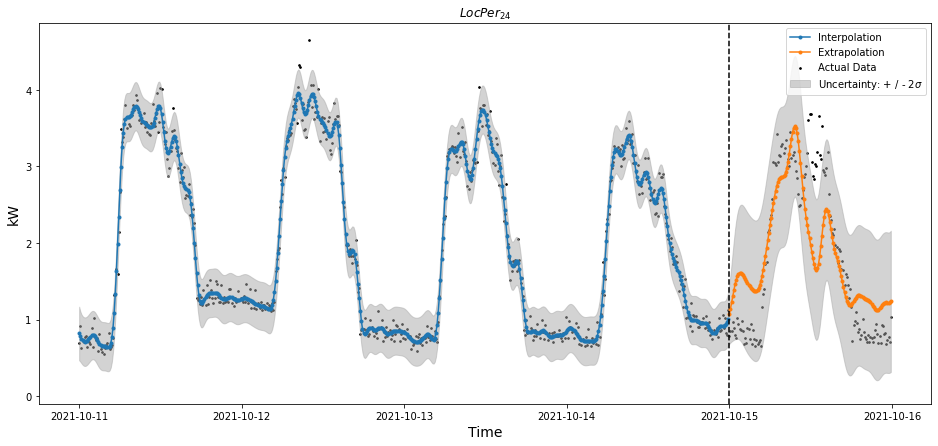
\includegraphics[scale=0.4]{images/LocPer24_entsorgung.png}\label{fig:a}} \\
    \subfloat[b][b]{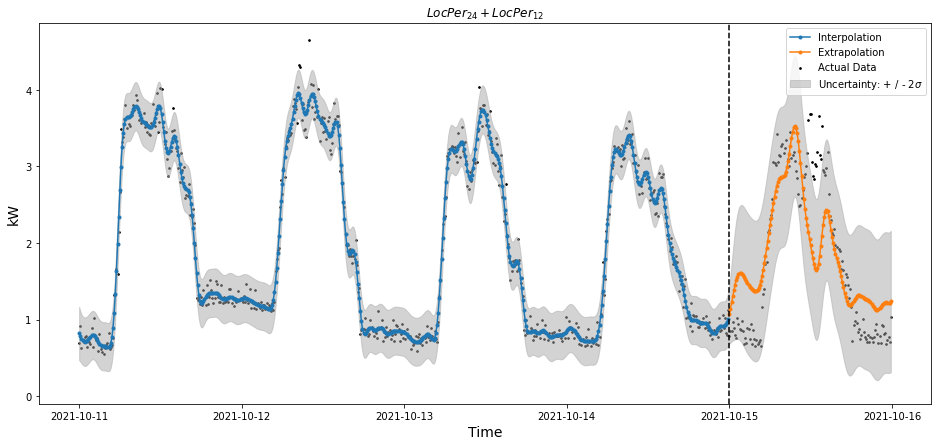
\includegraphics[scale=0.4]{images/LocPer24_LocPer12_entsorgung.png}\label{fig:b}} \\
    \subfloat[c][c]{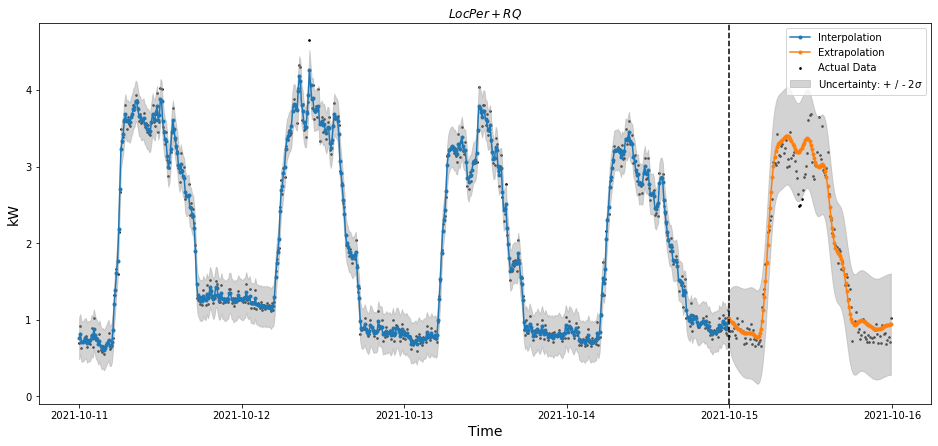
\includegraphics[scale=0.4]{images/LocPer_RQ_entsorgung.png}\label{fig:c}}
    \caption{Cumulatively adding more complex kernels. The dashed line represents the training and validation split. (a) $K_{LocPer24}$, (b) $K_{LocPer12}$, and (c) $K_{LocPer24} + K_{LocPer12} + K_{RQ}$}  \label{fig:AB}
    \label{fig:figure.13}
\end{figure}

\subsection{Optimization and Cross Validation}

Do I need this? (Probably....not)

\subsection{Energy Baseline Model Experiment Performance Metrics}

Following the kernel decomposition, the evaluation metrics are queried from the PostgreSQL database to determine which kernel design resulted in the best performance according to \hyperlink{subsection.3.7}{Section 3.7}. The result of this query is shown below.

\begin{table}[htbp]
\scalebox{0.81}{
    \renewcommand{\arraystretch}{1.2}
    \centering
    \begin{tabular}{lcccccccc}
    \hline
         Device & Aggregation & Kernel & MSE & MAPE & RMSE & ACE & Pinball  \\
    \hline
    Paper disposal 
     & $10$ & $K_{LocPer24} + K_{RQ}$ & $0.046$ & $0.117$ & $0.215$ & $0.99$ & $0.082$ \\
     & $30$ & $K_{LocPer24} + K_{RQ}$ & $0.032$ & $0.079$ & $0.179$ & $1.0$ & $0.062$ \\
     
    Gesamtmessung 
     & $10$ & $K_{LocPer24} + K_{LocPer12} + K_{RQ}$ & $169.354$ & $0.445$ & $13.014$ & $0.757$ & $4.913$ \\
     & $30$ & $K_{LocPer24} + K_{LocPer12} + K_{RQ}$ & $163.175$ & $0.447$ & $12.774$ & $0.771$ & $4.806$ \\
     
    eg 
     & $10$ & $K_{LocPer24} + K_{LocPer12} + K_{RQ}$ & $2.582$ & $0.117$ & $1.607$ & $0.80$ & $0.455$ \\
     & $30$ & $K_{LocPer24} + K_{LocPer12} + K_{RQ}$ & $2.63$ & $0.115$ & $1.622$ & $0.792$ & $0.443$ \\
     
    Hauptluftung 
     & $10$ & $K_{LocPer24} + K_{RQ}$ & $0.462$ & $0.132$ & $0.68$ & $0.931$ & $0.171$ \\
     & $30$ & $K_{LocPer24} + K_{RQ}$ & $0.287$ & $0.132$ & $0.536$ & $0.958$ & $0.173$ \\
     
    og 1 
     & $10$ & $K_{LocPer24} + K_{RQ}$ & $0.195$ & $0.178$ & $0.441$ & $0.965$ & $0.146$ \\
     & $30$ & $K_{LocPer24} + K_{RQ}$ & $0.162$ & $0.155$ & $0.402$ & $0.912$ & $0.132$ \\
     
    uv eg 
     & $10$ & $K_{LocPer24} + K_{LocPer12} + K_{RQ}$ & $2.599$ & $0.364$ & $1.612$ & $0.91$ & $0.457$ \\
     & $30$ & $K_{LocPer24} + K_{LocPer12} + K_{RQ}$ & $2.068$ & $0.296$ & $1.438$ & $0.917$ & $0.378$ \\
     
    \hline
    \end{tabular}}
    \caption{GP evaluation metrics for each machine and time aggregation. The learning rate was set to $0.1$, and the optimization loop consisted of $100$ iterations. The metrics in the table represent the lowest and or highest score achieved during the experimentation phase. For a full break of GP evaluation metrics, refer to the following table in the appendix.}
    \label{tab:my_label}
\end{table}

As expected, time aggregations of $30$ minutes typically results in lower MSE, MAPE, RMSE and pinball loss, and a higher ACE. The paper disposal machine has the best evaluation metrics at both $10$ and $30$ minute aggregations with og 1, HVAC, uv eg, and eg, following respectively. The main terminal is an interesting example. Referring to \textbf{figure 800} in the appendix, the baseline model predicted a longer duration load profile than what actually happened. Thus, the reason for the poor evaluation metrics. However, if more data was collected, it is likely possible the kernels will learn such a behavior. 